\chapter{\texorpdfstring{$\Omega$}{Omega}-\texorpdfstring{$\Pt$}{Pt} duality}\label{chap:Omega-Pt}
In this chapter we consider a Stone-type duality that applies to spaces more
general than the ones dual to distributive lattices. We begin
(Section~\ref{sec:StoneSpaces}) by showing how the ordered spaces in Priestley
duality for distributive lattices can be replaced by unordered topological
spaces. This recasting of Priestley duality uses the correspondence between compact ordered spaces and stably compact spaces already discussed in Section~\ref{sec:comp-ord-sp}. Then we introduce
an adjoint pair of functors (Section~\ref{sec:Omega-Pt-adjunction}) between the
category of topological spaces and a certain category of complete lattices. We
then show that this adjunction restricts to a duality between so-called sober
spaces and spatial frames (Section~\ref{sec:Omega-Pt-duality}). Finally, we give
a detailed description of how all these dualities fit together.


\section{Spectral spaces and Stone duality}\label{sec:StoneSpaces}
In the Priestley duality of Chapter~\ref{ch:priestley}, we obtain certain compact ordered spaces as duals of distributive lattices. However, in the original formulation by Stone, the dual spaces of distributive lattices are certain stably compact spaces (Definition~\ref{dfn:stab-comp-sp}). In fact the relationship between Stone's dual spaces and Priestley spaces is given by restricting the bijective correspondence between compact ordered spaces and stably compact spaces established in Theorem~\ref{thrm:COSpace-StabCompSp} of Chapter~\ref{chap:TopOrd}. The precise relationship between distributive lattices, Priestley spaces, and spectral spaces will be given in the commutative triangle of equivalences in Figure~\ref{fig:dl-priest-spec-diagram} below.


\begin{theorem}\label{thrm:Priestley-Stone}
Let $(X,\tau)$ be a stably compact space. The following statements are equivalent:
\begin{enumerate}
\item[(i)] $(X,\tau^p,\leq_\tau)$ is a Priestley space;
\item[(ii)] $(X,\tau^p,\geq_\tau)$ is a Priestley space;
\item[(iii)] $(X,\tau)$ has a basis of compact opens.
\item[(iv)] $(X,\tau^\partial)$ has a basis of compact opens.
\end{enumerate}
\end{theorem}

\begin{proof}
Since the definition of a Priestley space is self-dual with respect to order-duality, it follows that (i) and (ii) are equivalent. Since, under the correspondence of Theorem~\ref{thrm:COSpace-StabCompSp}, $(X,\tau)$ is the stably compact space corresponding to $(X,\tau^p,\leq_\tau)$ and $(X,\tau^\partial)$ is the stably compact space corresponding to $(X,\tau^p,\geq_\tau)$, it suffices to show that (iii) is equivalent to (i) and/or (ii) in order to show that all four statements are equivalent.

So suppose $(X,\tau)$ is a stably compact space for which $(X,\tau^p,\leq_\tau)$ is a Priestley space and let $x\in X$ and $U\in\tau$ with $x\in U$. We will construct a compact open set $V$ such that $x \in V \subseteq U$. Note that $C:=U^c$ is a closed downset which does not contain $x$. Hence, for each $y\in C$ we have $x\nleq y$ and thus there is a clopen upset $V_y$ of the Priestley space $(X,\tau^p,\leq_\tau)$ with $x\in V_y$ and $y\in V_y^c$. It follows that $\{V_y^c\}_{y\in C}$ is an open cover of $C$ in $(X,\tau^p,\leq_\tau)$. Since $C$ is closed and thus compact, it follows that there is a finite subset $F\subseteq C$ so that $\{V_y^c\}_{y\in F}$ is a cover of $C$. Consequently, the set
$V :=\bigcap\{V_y\mid y\in F\}$ 
is a clopen upset of $(X,\tau^p,\leq_\tau)$ with $x\in V\subseteq U$. Finally, since $V$ is an open up-set in $(X,\tau^p,\leq_\tau)$, it is open in the topology $(\tau^p)^{\uparrow}$, which is equal to $\tau$ by Proposition~\ref{prop:compordaspatch}. Also, since $V$ is closed in $(X,\tau^p,\leq_\tau)$, it is is compact in $(X,\tau^p,\leq_\tau)$, and thus also in the smaller topology of $(X,\tau)$, since the compact topologies are a down-set in $\Top(X)$ (Exercise~\ref{ex:down-and-up-in-Top}). We have thus shown that $(X,\tau)$ possesses a basis of compact opens.

For the converse, suppose $(X,\tau)$ is a stably compact space with a basis of compact opens, and let $x,y\in X$ with $x\nleq_\tau y$. By definition of the specialization order, it follows that there is an open $U\in\tau$ with $x\in U$ and $y\not\in U$. Also, since $(X,\tau)$ has a basis of compact opens, it follows that there is a compact open $V\subseteq X$ with $x\in V\subseteq U$. The fact that $V$ is open in $(X,\tau)$ implies that it is an open up-set in $(X,\tau^p,\leq_\tau)$. Furthermore, since $V$ is compact and open, and thus in particular saturated, it is closed in $(X,\tau^\partial)$, and thus also in $(X,\tau^p,\leq_\tau)$. Altogether, we have that $V$ is a clopen up-set in $(X,\tau^p,\leq_\tau)$ and that $x\in V$ and $y\not\in V$, as required.%
\end{proof}

We recall from Chapter~\ref{ch:priestley} that the morphisms of Priestley spaces are the continuous and order preserving maps, see also Example~\ref{exa:bigcats}. Thus, in order to obtain a (non-full) subcategory of $\TOP$ that is dual to the category of bounded distributive lattices, we have to consider the corresponding stably compact spaces with proper maps (see Exercise~\ref{exer:propermaps}). Finally, if $X$ and $Y$ are stably compact spaces satisfying the equivalent statements of Theorem~\ref{thrm:Priestley-Stone}, one can simplify the definition of proper maps: a map $f\colon X\to Y$ is a proper continuous map if and only if the pre-image of a compact-open is compact-open  (see Exercise~\ref{exer:Stone-maps}).

The above considerations naturally suggest the following definition of the category of \emph{spectral spaces}. A shorter but more ad hoc definition can be found in Exercise~\ref{exer:Stone-spaces}; alternative definitions in the literature often also explicitly include the statement that a spectral space is \emphind{sober} (see Definition~\ref{def:sober} below), but we will derive this as a consequence of our definition, see Exercise~\ref{exer:sober-vs-wellfiltered} below. The spaces we call spectral spaces are also known as \emphind{coherent spaces} or (non-Hausdorff) \emphind{Stone spaces} in less recent literature, but these terms have also been used with other meanings, so we will avoid using them\endnote{The name `Stone space' has also been used for the more restricted class of spaces that we call \emph{Boolean} spaces in this book. We prefer to avoid the name `Stone space' for a class of spaces, to avoid confusion. We do use the terminology `the Stone dual space of a lattice' to refer to the spectral space associated to a distributive lattice through Stone's duality.  Our choice of the terminology `spectral spaces' follows in particular the recent monograph \cite{DicSchTre2019}, the first chapters of which we recommend as useful complementary reading to the material in this chapter.}.
\begin{definition}\label{def:StoneSpace}
A \emphind{spectral space} is a stably compact space satisfying the equivalent statements of Theorem~\ref{thrm:Priestley-Stone}. We denote by $\Spec$ the category of spectral spaces with maps for which the pre-image of a compact-open is compact-open.
\end{definition}


\begin{definition}\label{def:StoneFunctor}
Let $L$ be a distributive lattice.  The \emph{Stone dual space of $L$} or \emph{spectral space of $L$}\index{Stone dual space of a lattice}\index{spectral space of a lattice}, denoted $\St(L)$, is a space $(X,\sigma)$, where $X$ comes with bijections $F_{(\ )}\colon X\to\PrFilt(L)$, $I_{(\ )}\colon X\to\PrIdl(L)$, $h_{(\ )}\colon X\to\Hom(L,\btwo)$ so that for all $x\in X$ and all $a\in L$ we have
\[
a\in F_x\quad\iff\quad a\not\in I_x \quad\iff\quad h_x(a)=\top,
\]
and the topology $\sigma$ is generated by the sets
\[
\eta(a)=\{x\in X\mid a\in F_x\}=\{x\in X\mid a\not\in I_x\}=\{x\in X\mid h_x(a)=\top\}
\]
where $a$ ranges over the elements of $L$. This object assignment extends to a contravariant functor
\[
\St\colon\DL\to\Spec
\]
where a homomorphism $h\colon L \to M$ is sent to the function  $f\colon X_M\to X_L$ given by
requiring that $F_{f(x)}=h^{-1}(F_x)$, for every $x \in X_M$.
\end{definition}

Given a topological space $X$ we denote by ${\KO}(X)$ the collection of compact-open subsets of $X$. Note that, if $(X,\sigma)$ is a spectral space with specialization order $\leq_\sigma$, then ${\KO}(X)$ ordered by inclusion is the distributive lattice which corresponds under Priestley duality to the Priestley space $(X,\sigma^p,\geq_\sigma)$, where we recall that $\sigma^p$ denotes the \emphind{patch topology}, i.e., the smallest topology containing both $\sigma$ and $\sigma^\partial$. Indeed, the clopen down-sets of $(X,\sigma^p, \geq_\sigma)$ are the clopen up-sets of $(X,\sigma^p, \leq_\sigma)$, which are exactly the compact open sets of $(X,\sigma)$ by Proposition~\ref{prop:with-without-order-scs}.\ref{itm:koisclup}. By definition, any proper continuous map $f \colon X \to Y$ yields a distributive lattice homomorphism $f^{-1} \colon {\KO}(Y) \to {\KO}(X)$. In summary, we have the following commutative triangle of categorical (dual) equivalences, where the equivalence between $\Priest$ and $\Spec$ is in fact an isomorphism, see Theorem~\ref{thm:Stone-isom-Priestley} below.

\begin{figure}[htp]
\begin{center}
\begin{tikzpicture}
  \node(DL) at (0,0) {$\DL^\op$};
  \node(Pr) at (4,2) {$\Priest$};
  \node(Sp) at (4,-2) {$\Spec$};
  
  \draw[->,>=stealth'] (DL) to[bend left=7] node[above] {$\mathrm{Pr}$} (Pr);
  \draw[->,>=stealth'] (Pr) to[bend left=7] node[below=.1] {$\ClD$} (DL);

  \draw[->,>=stealth'] (DL) to[bend left=10] node[above] {$\mathrm{Sp}$} (Sp);
  \draw[->,>=stealth'] (Sp) to[bend left=10] node[below=.1] {$\KO$} (DL);

  \draw[->,>=stealth'] (Pr) to[bend right=10] node[left] {$(\ )^{\downarrow}$} (Sp);
  \draw[->,>=stealth'] (Sp) to[bend right=10] node[right] {$\langle(\ )^{p},\geq_{(\ )}\rangle$} (Pr);
\end{tikzpicture}
\caption{A commutative triangle of equivalences. The equivalence between $\Priest$ and $\Spec$ is an isomorphism of categories, see Theorem~\ref{thm:Stone-isom-Priestley}. The dual equivalence between $\DL$ and $\Priest$ is the one described in Theorem~\ref{thm:priestley-duality-long}. The functors  between $\DL$ and $\Spec$ have been defined in this section; it is a dual equivalence because it is the composition of a dual equivalence with an isomorphism.}
\label{fig:dl-priest-spec-diagram}
\end{center}
\end{figure}



\begin{theorem}\label{thm:Stone-isom-Priestley}
  The categories {\Spec} and {\Priest} are isomorphic. On objects the isomorphisms are given, respectively, by the restriction of the patch construction for stably compact spaces, equipped with the reverse of the specialization order:
  \begin{align*}
    \langle(\ )^{p},\geq_{(\ )}\rangle \ \colon \ {\Spec}\  & \to {\Priest}\\
             (X,\sigma)\  & \mapsto (X,\sigma\vee\sigma^\partial, \geq_\sigma)
  \end{align*}
  and by intersecting with the dual Alexandrov topology of the order:
  \begin{align*}
  (\ )^{\downarrow}\colon {\Priest} & \to {\Spec}\\
             (X,\pi,\leq) & \mapsto (X,\pi\cap \Down(X,\leq)).
  \end{align*}
  On maps, the isomorphism of categories is simply the identity.
  \end{theorem}
  
  \begin{proof}
  By Theorem~\ref{thrm:Priestley-Stone} and the definition of spectral spaces, it follows that
  all spectral spaces are stably compact spaces and that the correspondence of Theorem~\ref{thrm:COSpace-StabCompSp}, applied with a reversal of the orderings, %
   between stably compact spaces and compact ordered spaces provides a bijective correspondence between spectral spaces and Priestley spaces. Furthermore, Exercise~\ref{exer:propermaps} shows that this bijective correspondence extends to an isomorphism of categories between the category {\Priest} and that of spectral spaces with proper maps. Finally, by Exercise~\ref{exer:Stone-maps}, proper maps between spectral spaces are precisely those for which the pre-image of a compact-open is compact-open, which in turn, by Definition~\ref{def:StoneSpace}, are the morphisms of the category {\Spec}.
   \end{proof}


\exercises

\begin{exercise}\label{exer:Stone-maps}
Show that a map between spectral spaces is proper if and only if the pre-image of a compact-open is compact-open. Further show that  a map between Boolean spaces is proper if and only if it is continuous.
\end{exercise}

\begin{exercise}\label{exer:non-proper}
  Show, by giving an example, that there may exist continuous maps $f\colon X\to Y$ between spectral spaces $X$ and $Y$ which are not proper.
  \end{exercise}

\begin{exercise}\label{exer:Stone-spaces}
Show that a topological space $X$ is a spectral space if and only if it is well filtered and ${\KO}(X)$ is a bounded sublattice of $\cP(X)$ and a basis for the topology of $X$.
\end{exercise}

\begin{exercise}\label{exer:Stone-duality}
Using Priestley duality, Theorem~\ref{thrm:COSpace-StabCompSp} of Chapter~\ref{chap:TopOrd}, and Theorem~\ref{thrm:Priestley-Stone} above, show that
\begin{enumerate}
\item The assignment $X\mapsto {\KO}(X)$ may be extended to a contravariant functor from $\Spec$ to $\DL$ by sending a proper map $f\colon X\to Y$ to the map
\[
\KO(f)\colon\KO(Y)\to\KO(X), \ U\mapsto f^{-1}[U].
\]
 \item The pair of functors $\St$ and $\KO$ yield a duality between the categories $\Spec$ and $\DL$.
\end{enumerate}
\end{exercise}


\begin{exercise}\label{exer:co-compactdualofStone}
  Show that if $(X,\sigma)$ is a spectral space, then the co-compact dual of $\sigma$ is generated by the complements of the compact-opens of $(X,\sigma)$. That is
  \[
  \sigma^\partial=\langle U^c\mid U\in\KO(X,\sigma)\rangle.
  \]
  \end{exercise}


\section{The \texorpdfstring{$\Omega$}{Omega}-\texorpdfstring{$\Pt$}{Pt} adjunction}\label{sec:Omega-Pt-adjunction}

The collection of open subsets of a topological space is closed under arbitrary unions and is thus a complete lattice in the inclusion order. If we restrict to the compact-open subsets of a spectral space, we obtain a collection of subsets closed just under finite intersections and finite unions and thus a distributive lattice. In fact, Stone duality tells us, among other things, that \emph{any} distributive lattice occurs as  $\KO(X)$ for an up to homeomorphism unique spectral space $X$.

Topological spaces that are not spectral spaces  will in general not have a basis of compact opens, but they will have lots of bases that  are bounded sublattices of the power set.\endnote{Using lattice bases of spaces, equipped with certain \emph{proximity} relations, leads to an alternative duality for stably compact spaces \cite{Smy92,JS96}.}
 If a compact space has a basis of compact opens, then, by compactness, this is necessarily the smallest basis which is closed under finite unions. Topological spaces that are not spectral spaces  will in general also not have a smallest bases. To obtain a canonical basis beyond spectral spaces, we are forced to take the basis of all opens. However, as noted above, this forces us to consider a category of complete lattices instead of the category of all distributive lattices.

\begin{definition}\label{def:frame}
A \emphind{frame} is a complete lattice in which finite meets distribute over infinite joins, that is, it satisfies the Join Infinite Distributive law (see (\ref{eq:JID})). A map between frames is said to be a \emphind{frame homomorphism} provided it preserves finite meets and arbitrary joins. We denote by $\Frame$ the category of frames with frame homomorphisms.
\end{definition}

\begin{example}\label{exa:frame-of-opens}
Given a topological space $X$, the collection of all opens is closed under binary intersections and arbitrary  unions. Since (arbitrary) intersections distribute over arbitrary unions, $\Omega(X)$ is a frame. Also, by the very definition of continuity, a continuous map $f\colon X\to Y$ yields a map
\[
\Omega(f)\colon\Omega(Y)\to \Omega(X)
\]
 given by $U\mapsto f^{-1}[U]$. Since the inverse image map preserves (arbitrary) intersections and arbitrary unions, the map $\Omega(f)$ is a frame homomorphism.
\end{example}

\begin{proposition}
$\Omega\colon\TOP\to\Frame$ is a contravariant functor.
\end{proposition}

\begin{proof}
It is straight forward to verify that $\Omega(\id_X)=\id_{\Omega(X)}$ for any topological space $X$, and that $\Omega(f\circ g)=\Omega(g)\circ\Omega(f)$ whenever $g\colon X\to Y$ and $f\colon Y\to Z$ are continuous maps.
\end{proof}

If we want a way to recapture a space from its frame of open sets, first, we need a way of distinguishing points using open sets. As soon as a space is $T_0$ this is possible via neighborhood filters.

\begin{definition}\label{def:neighborhood-filter}
Let $X$ be a topological space and $x\in X$. The \emphind{neighborhood filter} of $x$ is given by
\[
\cN(x)=\{ U\in\Omega(X)\mid x\in U\}.
\]
\end{definition}

\begin{definition}\label{def:compl-prime-filter}
Let $L$ be a frame. A subset $F\subseteq L$ is a \emphind{completely prime filter} of $L$ if it is a proper filter satisfying, for all $S\subseteq L$,
\[
\bigvee S\in F \quad\implies\quad S\cap F\neq\emptyset.
\]
We denote by $\CompPrFilt(L)$ the collection of all completely prime filters of $L$.
\end{definition}

The proof of the following proposition is left as Exercise~\ref{exer:proveNx}.

\begin{proposition}\label{prop:Nx}
Let $X$ be a topological space and $x\in X$. Then $\cN(x)$ is a completely prime filter in $\Omega(X)$.  
Furthermore, $X$ is $T_0$ if and only if the assignment $x\mapsto\cN(x)$ is injective.
\end{proposition}


Recall from Chapter~\ref{ch:order} that, for any distributive lattice $L$, $\M(L)$ denotes the set of meet-prime elements of $L$.

\begin{proposition}\label{prop:frame-points}
Let $L$ be a frame and $F\subseteq L$. The following statements are equivalent:
\begin{enumerate}[label=(\roman*)]
\item the set $F$ is a completely prime filter of $L$;
\item the complement $L\setminus F$ of $F$ is a principal down-set ${\downarrow}m$, for some $m \in \M(L)$;
\item the characteristic function $\chi_F\colon L\to \btwo$, where $\chi_F(a)=1$ if and only if $a\in F$, is a frame homomorphism.
\end{enumerate}
\end{proposition}

\begin{proof}
First suppose $F$ is a completely prime filter of $L$. Define $m:=\bigvee (L\setminus F)$. Clearly, $L\setminus F\subseteq{\downarrow}m$. Since $F$ is completely prime and $(L\setminus F)\cap F=\emptyset$, it follows that $m\not\in F$. Therefore, since $L\setminus F$ is a down-set, $
{\downarrow}m\subseteq L\setminus F$, 
and thus ${\downarrow}m=L\setminus F$. Finally, for any finite $M\subseteq L$, if  $\bigwedge M\leq m$, then $\bigwedge M\not\in F$, because $m \not\in F$ and $F$ is an up-set. So there is $m'\in M$ with $m'\not\in F$ or equivalently $m'\leq m$. Thus, $m \in \M(L)$, and we have shown that (i) implies (ii).

Now suppose that $L\setminus F={\downarrow}m$ for some $m \in \M(L)$. To see that $\chi_F$ preserves arbitrary joins, note that, for any $A \subseteq L$, $\chi_F(\bigvee A) = 1$ if, and only if, $\bigvee A \nleq m$, if, and only if, $a \nleq m$ for some $a \in A$, which is equivalent to $\bigvee \chi_F[A] = 1$. %
That $\chi_F$ preserves finite meets follows directly from the definition of meet-prime: for any finite $A \subseteq L$, $\chi_F(\bigwedge A) = 1$ if, and only if, $\bigwedge A \nleq m$, which, since $m \in \M(L)$, happens if, and only if, $a \nleq m$ for every $a \in A$, and this is in turn equivalent to $\bigwedge \chi_F[A] = 1$.

For the last implication, suppose that $\chi_F\colon L\to \btwo$ is a frame homomorphism. Since $\chi_F$ preserves finite meets, it follows that $F=\chi_F^{-1}(1)$ is a filter. If $A\subseteq L$ with $\bigvee A\in F$, then $\chi_F(\bigvee A)=1$ and thus $\chi_F(a)=1$ for some $a\in A$. That is, $A\cap F\neq\emptyset$ and thus $F$ is completely prime.
\end{proof}

We are now ready to give the definition of the $\Pt$ functor which takes us from frames back to topological spaces. The \emph{space of points} of a frame may be seen as based on the set of homomorphisms into the frame $\btwo$ or on the set of completely prime filters. We give both descriptions here leaving it as an exercise to check the details and the equivalence of the two descriptions, since the proofs are very similar to those already given in Section~\ref{sec:topologize} for Priestley duality. Note, however, that we only obtain a contravariant adjunction here; we will show how it restricts to a duality in the next section.

\begin{definition}\label{def:Pt-functor}
Given a frame $L$, we denote by $\Pt(L)$ a topological space which is determined up to homeomorphism by the fact that it comes with two bijections $F\colon\Pt(L)\to \CompPrFilt(L)$ and $f_{(\ )}\colon\Pt(L)\to\Hom_\Frame(L,\btwo)$ satisfying
\[
\forall x\in\Pt(L)\quad\forall a\in L\qquad (\ a\in F(x)\quad\iff\quad f_x(a)=1\ ),
\]
and the opens of $\Pt(L)$ are the sets
\[
\widehat{a}=\{x\in\Pt(L)\mid a\in F(x)\}.%
\]
where $a$ ranges over the elements of $L$.

The assignment $L\mapsto\Pt(L)$ extends to a contravariant functor
\[
\Pt\colon\Frame\to\TOP
\]
by sending a frame homomorphism $h\colon L\to M$ to the continuous map $\Pt(h)\colon\Pt(M)\to\Pt(L)$ given by
\begin{align*}
\Pt(h)(x)=y\quad &\iff\quad h^{-1}( F(y))= F(x)\\
                           &\iff\quad f_y=f_x\circ h.
\end{align*}
\end{definition}

\begin{theorem}\label{thrm:OmegaPoint-adjunction}
The functors $\Pt\colon\Frame\rightleftarrows\TOP\colon\Omega$ form a contravariant adjunction with corresponding natural transformations given, for $L$ a frame, by
\begin{align*}
\eta_L\colon & L\to \Omega(\Pt(L))\\
         a          &\mapsto \{x\in\Pt(L)\mid a\in  F(x)\}
\end{align*}
and, for $X$ a topological space,
\begin{align*}
\varepsilon_X\colon & X\to \Pt(\Omega(X))%
\end{align*}
sends an element of $X$ to the element of $\Pt(\Omega(X))$ which corresponds to the neighborhood filter of $x$.
\end{theorem}

\begin{proof}
In order to check that the pair $(\Pt,\Omega)$ forms an adjunction it suffices to check that, for each frame homomorphism $h\colon L\to M$ and each continuous map $f\colon X\to Y$, the following diagrams commute
\[
\begin{tikzpicture}
\node(PY) at (0,1.5) {$L$};
\node(PX) at (3,1.5) {$\Omega(\Pt(L))$};
\node(OY) at (0,0) {$M$};
\node(OX) at (3,0) {$\Omega(\Pt(M))$};

\draw[->,>=stealth'] (PY)to node[above] {$\eta_L$} (PX);
\draw[->,>=stealth'] (OY) to node[below] {$\eta_M$} (OX);
\draw[->,>=stealth'] (PY) to node[left] {$h$}(OY);
\draw[->,>=stealth'] (PX) to node[right]  {$\Omega(\Pt(h))$}(OX);
\end{tikzpicture}
\qquad
\begin{tikzpicture}
\node(PY) at (0,1.5) {$X$};
\node(PX) at (3,1.5) {$\Pt(\Omega(X))$};
\node(OY) at (0,0) {$Y$};
\node(OX) at (3,0) {$\Pt(\Omega(Y))$};

\draw[->,>=stealth'] (PY)to node[above] {$\varepsilon_X$} (PX);
\draw[->,>=stealth'] (OY) to node[below] {$\varepsilon_Y$} (OX);
\draw[->,>=stealth'] (PY) to node[left] {$f$} (OY);
\draw[->,>=stealth'] (PX) to node[right]  {$\Pt(\Omega(f))$}(OX);
\end{tikzpicture}
\]



We leave these verifications as an exercise for the reader.
\end{proof}

\exercises
\begin{exercise}
Give an example of a topological space $X$ such that:
\begin{enumerate}
\item $\Omega(X)$ is not closed under arbitrary intersections;
\item $\Omega(X)$ does not satisfy the Meet Infinite Distributive law (order dual of JID);
\item There is a frame homomorphism from $\Omega(X)$ into $\btwo$ which does not preserve arbitrary meets.
\end{enumerate}
\end{exercise}


\begin{exercise}\label{exer:infimum-in-frame}
Let $X$ be a topological space and let $L = \Omega(X)$. Prove that, for any $S \subseteq L$, the infimum of $S$ is the interior of the set $\bigcap_{U \in S} U$, i.e., $\bigwedge S = \int(\bigcap S)$.
\end{exercise}

\begin{exercise}
  \label{exer:proveNx}
Prove Proposition~\ref{prop:Nx}.
\end{exercise}

\begin{exercise}\label{exer:pt-functor}
Show that $\Pt(L)$ is well-defined and that it is a topological space. Also show that the bijection $f_{(\ )}\colon\Pt(L)\to\Hom_\Frame(L,\btwo)$ embeds $\Pt(L)$ as a closed subspace of the space $\btwo^L$, where $\btwo$ has the Sierpinski topology (see Exercise~\ref{ex:Sierpinski}). Further, show that $\Pt(h)$ is well-defined and that it is a continuous map. Finally show that $\Pt$ is a contravariant functor as stated in Definition~\ref{def:Pt-functor}.
\end{exercise}

\begin{exercise}
Prove Theorem~\ref{thrm:OmegaPoint-adjunction}.
\end{exercise}




\section{The \texorpdfstring{$\Omega$}{Omega}-\texorpdfstring{$\Pt$}{Pt} duality}\label{sec:Omega-Pt-duality}
Recall from Corollary~\ref{cor:restricttoduality} that any contravariant adjunction, such as the one given by the functors $\Pt$ and $\Omega$ in the previous section, restricts to a maximal duality. This associated duality is obtained by restricting the functors to the full subcategories given by the objects for which the natural map from the object to its double dual is an isomorphism. 

Accordingly we want to characterise those frames for which $\eta_L\colon L\to\Omega(\Pt(L))$ is an isomorphism and those topological spaces for which $\varepsilon_X\colon X\to\Pt(\Omega(X))$ is a homeomorphism.

\begin{proposition}\label{prop:spatial}
Let $L$ be a frame. The following statements are equivalent:
\begin{enumerate}[label=(\roman*)]
\item $\eta_L\colon L\to\Omega(\Pt(L))$ is an isomorphism;
\item $\eta_L$ is injective;
\item For all $a,b\in L$, if $b\nleq a$ then there is $x\in\Pt(L)$ with $b\in F(x)$ and $a\not\in F(x)$;
\item For all $a\in L$, \quad $a=\bigwedge(\M(L)\cap{\uparrow} a).$
\end{enumerate}
\end{proposition}

\begin{proof}
By definition of $\Pt(L)$, the opens of this space are precisely the sets in the image of $\eta_L$ and thus $\eta_L$ is always surjective. It follows that items (i) and (ii) are equivalent since a frame homomorphism is an isomorphism if and only if it is both injective and surjective.

Further, since $\eta_L$ is always a frame homomorphism, it is always order preserving. Thus, all that is needed for injectivity (or equivalently order embedding, see Exercise~\ref{exe:injlatthom}) is that $\eta_L$ is order reversing. But (iii) is exactly the contrapositive of the statement that $\eta_L$ is order reversing.

We use Proposition~\ref{prop:frame-points} to prove the equivalence of (iii) and (iv).

In order to prove that (iii) implies (iv), we reason by contraposition:  suppose that (iv) fails, we show that (iii) also fails. Denote by $b$ the element $\bigwedge (\M(L) \cap {\uparrow}a)$. We must then have $b \nleq a$, since $a \leq b$ always holds. Let $x \in \Pt(L)$ be arbitrary such that $b \in F(x)$ and, by Proposition~\ref{prop:frame-points}, pick $m \in \M(L)$ such that $F(x) = ({\downarrow}m)^c$. Then $b \nleq m$, so in particular $a \nleq m$, by the very definition of $b$. Thus, $a \in F(x)$. Since $x$ was arbitrary, this shows that (iii) also fails.

For the converse, suppose  (iv) holds and let $a,b\in L$ with $b\nleq a$. Since  $a=\bigwedge(\M(L)\cap{\uparrow} a)$, we have $b\nleq\bigwedge(\M(L)\cap{\uparrow} a)$ and thus there is $m\in\M(L)$ with $a\leq m$ but $b\nleq m$. Again by Proposition~\ref{prop:frame-points}, $F=({\downarrow}m)^c$ is a completely prime filter of $L$, and thus there is an $x\in\Pt(L)$ with $F(x)=F$. It follows that $b\in F(x)$ and $a\not\in F(x)$ and thus (iii) holds.
\end{proof}

\begin{remark}
As we saw in Section~\ref{sec:finDLduality}, in a finite distributive lattice, each element is a finite join of join irreducible elements and a finite meet of meet irreducible elements. This is not the case for frames in general (see Exercise~\ref{exer:meet-irred}).
\end{remark}

\begin{definition}\label{def:spatial}
A frame is said to be \emphind{spatial} provided it satisfies the equivalent conditions of Proposition~\ref{prop:spatial}. We denote by {\SpFrame} the full subcategory of {\Frame} given by the spatial frames.
\end{definition}

As we have already observed, the natural morphism $\varepsilon_X\colon X\to\Pt(\Omega(X))$ is injective if and only if $X$ is a $T_0$ space.

\begin{proposition}\label{prop:sober}
Let $X$ be a $T_0$ space. The following statements are equivalent:
\begin{enumerate}[label=(\roman*)]
\item $\varepsilon_X\colon X\to\Pt(\Omega(X))$ is a homeomorphism;
\item $\varepsilon_X$ is surjective;
\item For all $y\in\Pt(\Omega(X))$ there is an $x\in X$ so that  $ F(y)=\cN(x)$;
\item The join irreducible elements of the lattice $\cC(X)$ of closed sets in $X$ are precisely the closures of points, $\overline{\{x\}}={\downarrow} x$, for $x\in X$.
\end{enumerate}
\end{proposition}

\begin{proof}
Recall that the opens of $\Pt(\Omega(X))$ are, by definition, the sets of the form $\widehat{U}=\{y\in\Pt(L)\mid U\in F(y)\}$, where $U \in \Omega(X)$. We have, for any $x \in X$ and $U \in \Omega(X)$,
\begin{align*}
\varepsilon_X(x)\in \widehat{U} & \iff U\in F(\varepsilon_X(x))=\cN(x)\\
						& \iff x\in U.
\end{align*}
Thus $\varepsilon_X$ is always an open continuous embedding of topological spaces and therefore it is clear that (i) is equivalent to (ii). Also, by definition of $\varepsilon_X$, an $x\in X$ is sent to the unique element $y\in\Pt(\Omega(X))$ with the property that $F(y)=\cN(x)$. Thus (iii) is simply spelling out the statement that $\varepsilon_X$ is surjective and therefore (ii) and (iii) are equivalent.

To prove that (iii) implies (iv), suppose that (iii) holds and let $C\in\cC(X)$ be join irreducible. Then, since the lattice of closed sets of $X$ is order dual to the lattice of open sets of $X$, we have that $U=C^c$ is a meet irreducible element of the frame $\Omega(X)$. By Proposition~\ref{prop:frame-points}, it follows that the set
\[
F_C=({\downarrow}U)^c=\{V\in\Omega(X)\mid V\not\subseteq U\}=\{V\in\Omega(X)\mid C\cap V\neq \emptyset\}
\]
is a completely prime filter of $\Omega(X)$. Now let $y\in\Pt(\Omega(X))$ be the point of $\Omega(X)$ corresponding to $F_C$, that is, the point with $F(y)=F_C$. Since (iii) holds, there is $x\in X$ with $F_C=\cN(x)$. That is, for all $V\in\Omega(X)$ we have
\[
C\cap V\neq \emptyset \quad\iff\quad x\in V.
\]
We use this to show that $C=\overline{\{x\}}$. To this end let $D$ be any closed subset of $X$ and let $V=D^c$ be the complementary open set. Then we have the following string of equivalences
\[
C\subseteq D\iff C\cap V=\emptyset \iff x\not\in V \iff x\in D.
\]
Thus we obtain the desired conclusion
\[
C=\bigcap\{D\in\cC(X)\mid C\subseteq D\}=\bigcap\{D\in\cC(X)\mid x\in D\}=\overline{\{x\}}
\]
and every join irreducible closed set is the closure of a singleton. The fact that closures of singletons always are join irreducible in the lattice of closed sets is left for the reader as Exercise~\ref{ex:singleton-joinirr}. 

To prove that (iv) implies (iii), let $y\in\Pt(\Omega(X))$ and let $F=F(y)$ be the corresponding completely prime filter of $\Omega(X)$. By Proposition~\ref{prop:frame-points}, the complement of $F$ is the down-set of some open set $U$ which is meet irreducible in the lattice $\Omega(X)$. It follows that $C=U^c$ is a closed subset of $X$ which is join irreducible in the lattice $\cC(X)$ of closed sets in $X$. By (iv), there exists $x\in X$ with $C=\overline{\{x\}}$. Now let $V\in\Omega(X)$, then we have
\[
V\not\in F \iff V\subseteq U\iff C\cap V=\emptyset \iff \overline{\{x\}}\cap V=\emptyset \iff x\not\in V
\]
and thus $V\in F$ if and only if $x\in V$ so that $F=\cN(x)$ as required.
\end{proof}

\begin{definition}\label{def:sober}
A topological space is said to be \emphind{sober} provided it is a $T_0$ space and  satisfies the equivalent conditions of Proposition~\ref{prop:sober}. We denote by {\SOB} the full subcategory of {\TOP} given by the sober topological spaces.
\end{definition}

It now follows, using Corollary~\ref{cor:restricttoduality}, that the functors $\Omega$ and $\Pt$, properly restricted and co-restricted, yield a duality between the category of spatial frames and the category of sober spaces.

\begin{theorem}\label{thrm:Omega-Point-duality}
The $\Omega$-$\Pt$ adjunction cuts down to a duality between the category of spatial frames with frame homomorphisms and the category of sober topological spaces with continuous maps.
\[
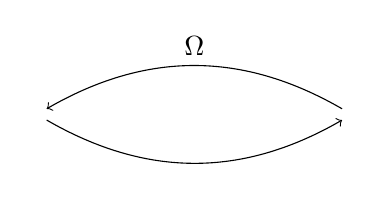
\begin{tikzpicture}
  \node (A) {{\SpFrame}};
  \node (B) [node distance=4cm, right of=A] { {\SOB}};
  \draw[->,bend right] (A) to node [above,midway] {$\Pt$} (B);
  \draw[->, bend right] (B) to node [above,midway]{$\Omega$} (A);
\end{tikzpicture}
\]
\end{theorem}
We end this chapter with a summary of the relationship between the $\Omega$-$\Pt$, the Stone, and the Priestley dualities. Recall that we already showed how Stone and Priestley duality for distributive lattices relate in Figure~\ref{fig:dl-priest-spec-diagram}. We now add the $\Omega$-$\Pt$ duality into the mix.

Since the $\Omega$-$\Pt$ duality is for unordered topological spaces rather than ordered spaces, we compare it to Stone duality rather than to Priestley duality. As we have seen in Exercise~\ref{exer:sober-vs-wellfiltered}, every spectral space is sober, thus {\Spec} is a subcategory of {\SOB}. Note that it is not a full subcategory, since not every continuous map between spectral spaces is proper; see Exercise~\ref{exer:non-proper}. Also, Exercise~\ref{exer:join-approx} outlines a generalization of Stone duality for the category $\Spec_c$ of spectral spaces with continuous, rather than spectral functions -- the dual category of distributive lattices then has certain relations as its morphisms.

The $\Omega$-$Pt$ duality is not directly a generalisation of Stone duality as, under the $\Omega$-$Pt$ duality, a spectral space is sent to its entire open set lattice rather than just to the lattice of compact-opens. However, the category $\DL$ embeds into the category $\Frame$ via the \emph{ideal completion} $A\mapsto \Idl(A)$, which freely adds directed joins to $A$. A \emphind{compact} element $k$ of a frame $F$ is one such that, for every directed subset $S$ of $F$, we have $k\leq\bigvee S$ implies $k\leq s$ for some $s\,{\in}\, S$, also see Section~\ref{sec:dom} for more on compact elements in the more general setting of directedly complete posets. We denote by $\Comp(F)$ the set of compact elements of $F$, which always forms a join-subsemilattice. In $\Idl(A)$, the compact elements are the principal ideals, thus we have $A\cong \Comp(\Idl(A))$. Finally, calling \emph{arithmetic frames} those frames whose compact elements form a sublattice which generates the frame by directed joins, we obtain the following diagram (Figure~\ref{fig:stone-omega-pt-objects}) which illustrates how to move back and forth between the Stone duality and the $\Omega$-$\Pt$ duality.
\begin{figure}[htp]
  \begin{center}
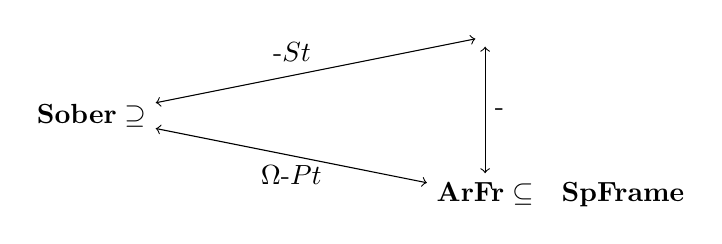
\begin{tikzpicture}
  \node (A) {$\mathbf{Sober}\supseteq \Spec$};
  \node (B) [node distance=5cm, yshift=1cm, right of=A] {${\DL}$};
  \node (C) [node distance=5cm, yshift=-1cm, right of=A] {$\mathbf{ArFr}\subseteq $};
  \node (C') [node distance=1.75cm, right of=C]{$\mathbf{SpFrame}$};
  \draw[<->] (B) to node [right,midway]{$\Idl$-$\Comp$} (C);
  \draw[<->] (A) to node [above,midway] {${\KO}$-$St$\hspace*{.6cm}} (B);
  \draw[<->] (A) to node [below,midway]{$\Omega$-$Pt$} (C);
\end{tikzpicture}
\end{center}
\caption{Comparing the $\Omega$-$\Pt$ and Stone duality on objects.}
\label{fig:stone-omega-pt-objects}
\end{figure}


\noindent This diagram is not the whole story as it does not specify what happens with morphisms. Stone duality acts on maps in $\Spec$, which is not a full subcategory of the category $\SOB$ of sober spaces with continuous maps. The $\Omega$-$\Pt$ duality, on the other hand, works on the full subcategory given by the spectral spaces. To get the maps dual to the proper maps we need to restrict the frame homomorphisms between arithmetic frames to those that carry compact elements to compact elements. An alternative way of seeing this is bitopological: a function between lattices is a homomorphism if and only if it is a homomorphism between the order duals of the two lattices. In fact lattice homorphisms correspond precisely to those continuous maps between spectral spaces that are also continuous with respect to the co-compact dual spectral topologies. Working with spectral spaces equipped with \emph{both} these topologies and the  corresponding notion of frames, one gets a natural bitopological description of lattice homomorphisms, see \cite{JuMo06}.
Alternatively to restricting the morphisms on the spectral spaces and arithmetic frames to fit those of bounded distributive lattices, we can weaken the notion of morphism on ${\DL}$ to correspond to lattice homomorphisms $A\,{\to}\, Idl(B)$, which in turn may be seen as certain `join-approximable' relations from $A$ to $B$, see Exercise~\ref{exer:join-approx} below.

\exercises



\begin{exercise}\label{exer:meet-irred}
Give an example of an infinite frame in which each element is a finite meet of meet irreducible elements and one in which it is not the case.
\end{exercise}

\begin{exercise}\label{exer:non-spatial}
This exercise contains material beyond the scope of this book. It is given mainly as an indication of a means of getting one's hands on non-spatial frames.
\begin{enumerate}
\item Show that non-atomic complete Boolean algebras are examples of non-spatial frames. To this end you may proceed as follows.
\begin{enumerate}[label=(\arabic*)]
\item Every complete Boolean algebra is a frame, that is, it satisfies (JID);
\item A complete Boolean Algebra is a spatial frame if and only if  it is \emphind{atomic} i.e., for all $b,c\in B$, if $b\nleq c$ then there is an atom $a$ of $B$ with $a\leq b$ but $a\nleq c$.
\end{enumerate}
\item Show that there exist non-atomic complete Boolean algebras. To this end you may proceed via (1)--(3) or via (4) below.
\begin{enumerate}[label=(\arabic*)]
\item There exist non-atomic Boolean algebras (e.g. the Lindenbaum-Tarski algebra of Classical Propositional Logic on a countable set of primitive propositional variables, see Section~\ref{sec:free-description}, has no atoms at all).
\item The MacNeille completion \cite{Mac37} of a Boolean algebra is atomic if and only if the original Boolean algebra is atomic.
\item There exist non-atomic complete Boolean algebras (e.g. the MacNeille completion of the Lindenbaum-Tarski algebra of Classical Propositional Logic on a countable set of primitive propositional variables).
\item Alternatively, one can show that the regular open subsets of a Hausdorff space form a complete Boolean algebra, where we recall that an open subset in a topological space is called \emph{regular} if it is equal to the interior of its closure. Further, if the original space has no isolated points then the Boolean algebra of regular opens has no atoms and is thus non-atomic.
\end{enumerate}
\end{enumerate}
\end{exercise}

\begin{exercise}\label{exer:non-sober}
  Show that, if $X$ is an infinite set equipped with the topology generated by the cofinite subsets, then $X$ is $T_0$, but not sober.
\end{exercise}

\begin{exercise}\label{exer:sobriety}
Show that all Hausdorff spaces are sober but that some $T_1$ spaces are not.
\end{exercise}
\begin{exercise}\label{ex:singleton-joinirr}
  Let $X$ be a topological space.
  Prove that the closure of a singleton set is join-irreducible in the lattice of closed subsets of $X$.
\end{exercise}
\begin{exercise}\label{exer:sober-vs-wellfiltered}
Show that if $X$ is a locally compact space, then $X$ is well filtered if and only if it is sober. Use this in combination with Exercise~\ref{exer:Stone-spaces} to show that a $T_0$ topological space is a spectral space if and only if the following two properties hold:
\begin{enumerate}
\item The collection of compact-open subsets of $X$ form a bounded sublattice of $\cP(X)$ and a basis for the topology of $X$;
\item $X$ is sober.
\end{enumerate}
\end{exercise}

\begin{exercise}\label{exer:sober-and-order}
Let $L$ be a frame.
\begin{enumerate}
\item Show that for $x,y\in \Pt(L)$ we have $x\leq y$ in the specialization order if and only if $f_x\leq f_y$ if and only if $F(x)\leq F(y)$;
\item Show that binary joins and meets need not exist in a sober space;
\item Show that the poset of completely prime filters of a frame is closed under directed union. Conclude that any sober space is a dcpo in its specialization order %(see Proposition~\ref{prop:sober-vs-dcpo} for a direct proof, not using the $\Omega$-$\Pt$ duality)
;
\item Show that each open of $\Pt(L)$ is Scott open with respect to the specialization order of $\Pt(L)$ %(again, see Proposition~\ref{prop:sober-vs-dcpo} for a direct proof of this fact for sober spaces)
.
\end{enumerate}
\end{exercise}

\begin{exercise}\label{exer:join-approx}
Let $L$ and $M$ be distributive lattices. A relation $R\subseteq L\times M$ is called \emph{join-approximable} (see, e.g., \cite[Definition~7.2.24]{AbJu94}) provided that, for any $a, a' \in L$ and $b, b' \in M$, the following four properties hold hold: (i) if $a' \geq a {R} b \geq b'$, then $a' {R} b'$; (ii) if $aRb$ and $aRb'$ then $a{R}b \vee b'$; (iii) if $a{R}b$ and $a'{R}b$ then $a \wedge a'{R} b$; (iv) if $a \vee a' {R} b$ then there exist $c, c' \in K$ such that $a{R}c$, $a'{R}c'$, and $b \leq c \vee c'$.

Denote by $X$ and $Y$ the spectral spaces dual to $L$ and $M$, respectively.
\begin{enumerate}
\item Show that there is a one-to-one correspondence between continuous functions $f\colon Y\to X$ and {\DL} homomorphisms $h\colon L\to \Idl(M)$.

\hint{Use the fact that $\Omega(X)$ is isomorphic to $\Idl(M)$.}
\item Show that there is a one-to-one correspondence between {\DL} homomorphisms $h\colon L\to \Idl(K)$ and join-approximable relations $R\subseteq L\times K$.
\item Conclude that the category of distributive lattices with join-approximable relations as the morphisms is dually equivalent to the category of spectral spaces with continuous functions between them. 
\end{enumerate}
\end{exercise}





\theendnotes
\setcounter{endnote}{0}

